% !TeX root = ../sustechthesis-example.tex

\chapter[几种构想的机器人类型草图]{几种构想的机器人类型草图}
\begin{figure}
  \centering
  \subcaptionbox{Wheeled humanoid\label{fig:a_wheeled_humanoid}}
    {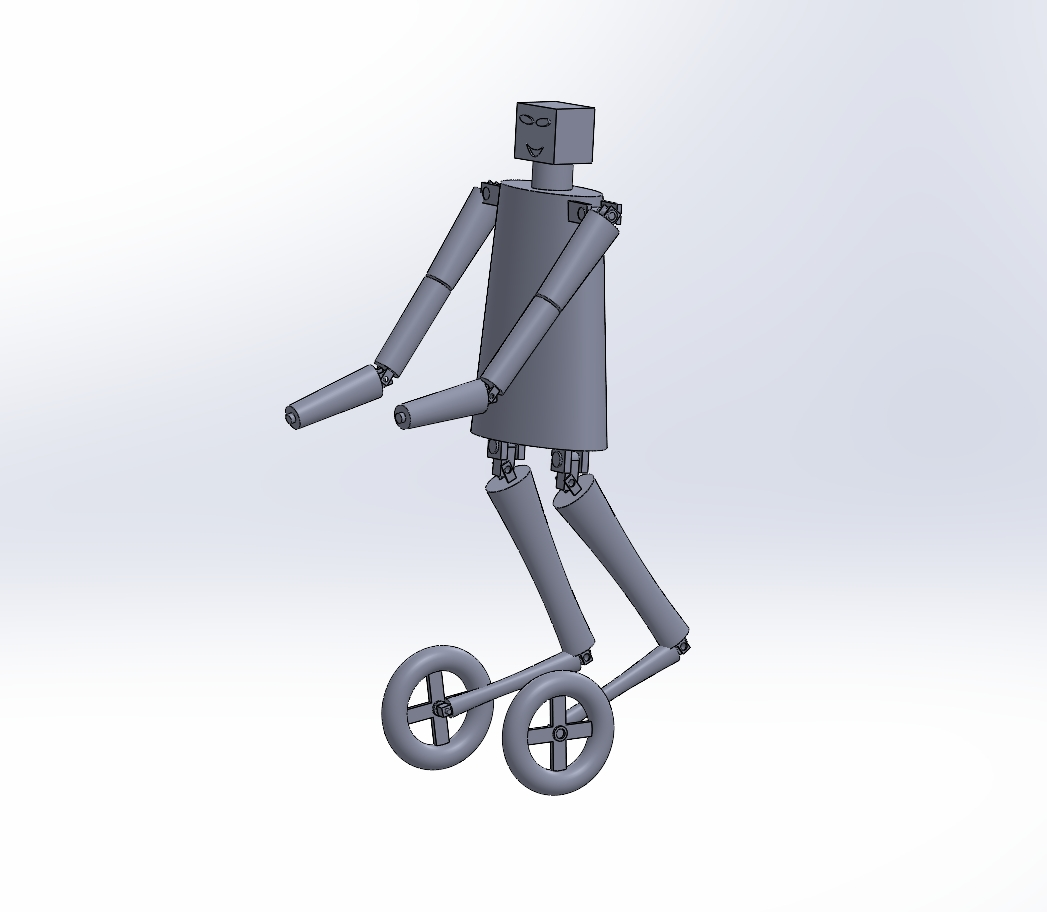
\includegraphics[width=0.3\linewidth]{wheeled_humanoid.png}}
  \subcaptionbox{Roller humanoid\label{fig:b_roller_humanoid}}
    {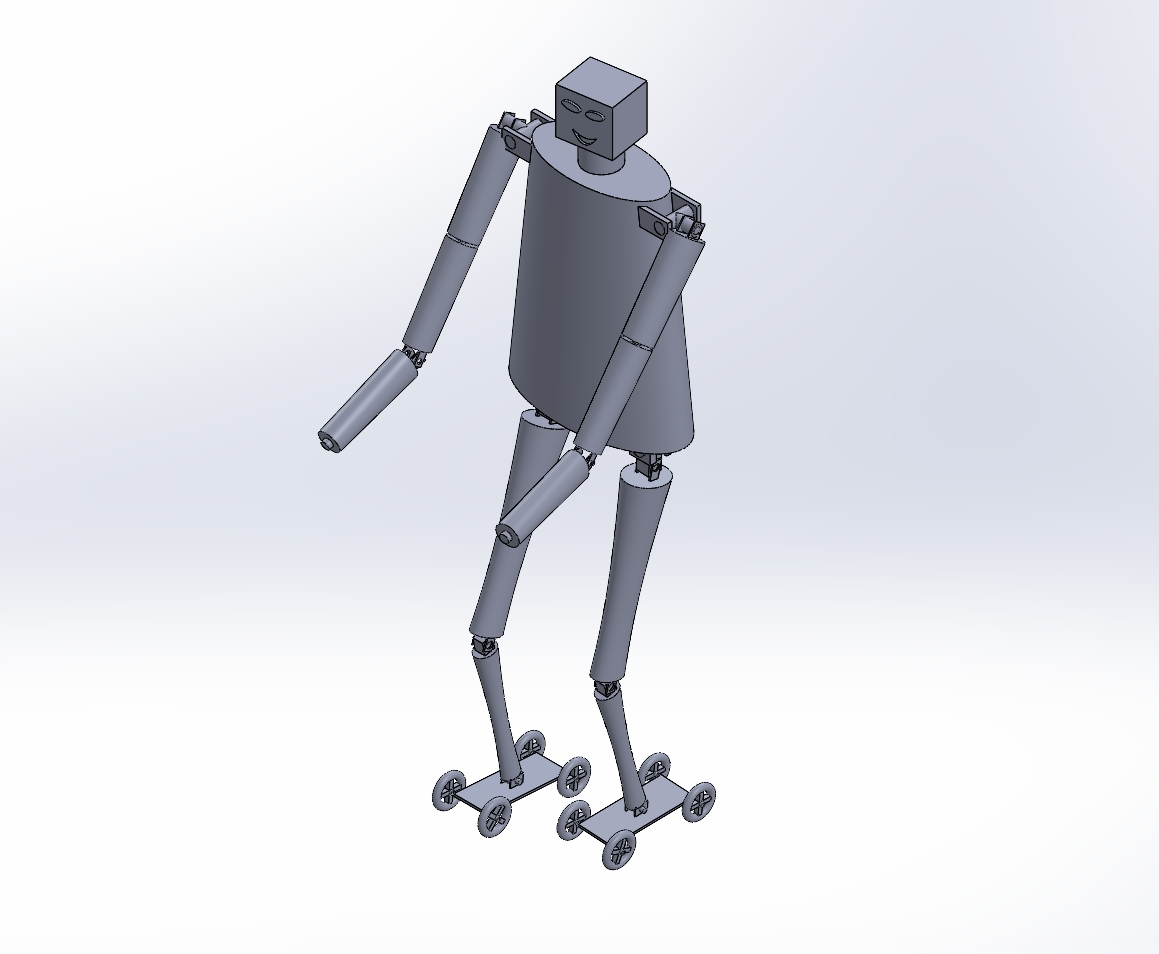
\includegraphics[width=0.3\linewidth]{roller_humanoid.png}}
  \subcaptionbox{wheeled flying\label{fig:c_wheeled_flying}}
    {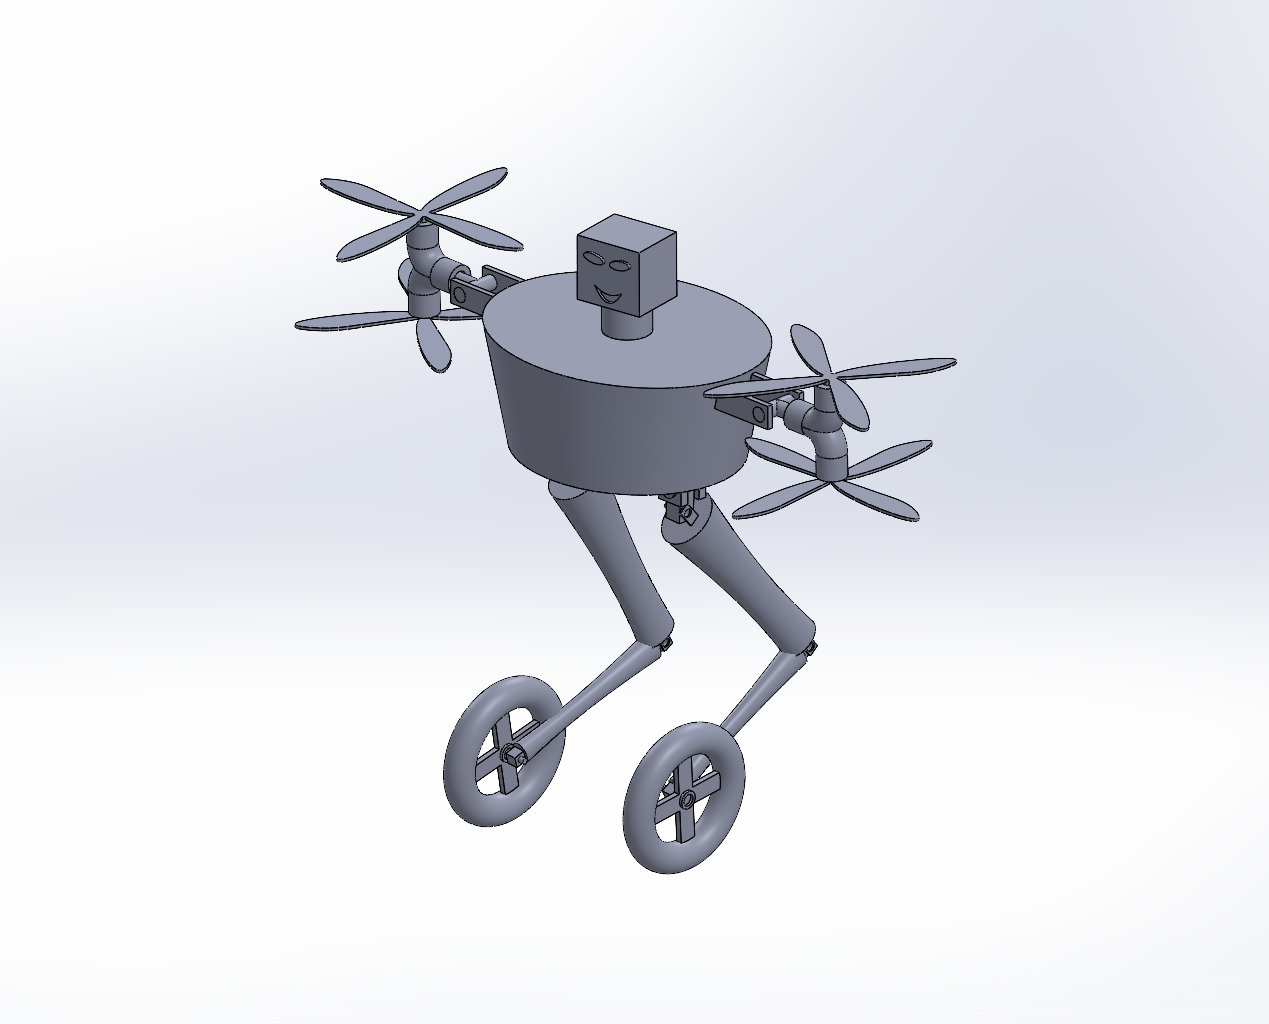
\includegraphics[width=0.3\linewidth]{wheeled_flying.png}}
  % \subcaptionbox{分图 D\label{fig:subfig-d}}
  %   {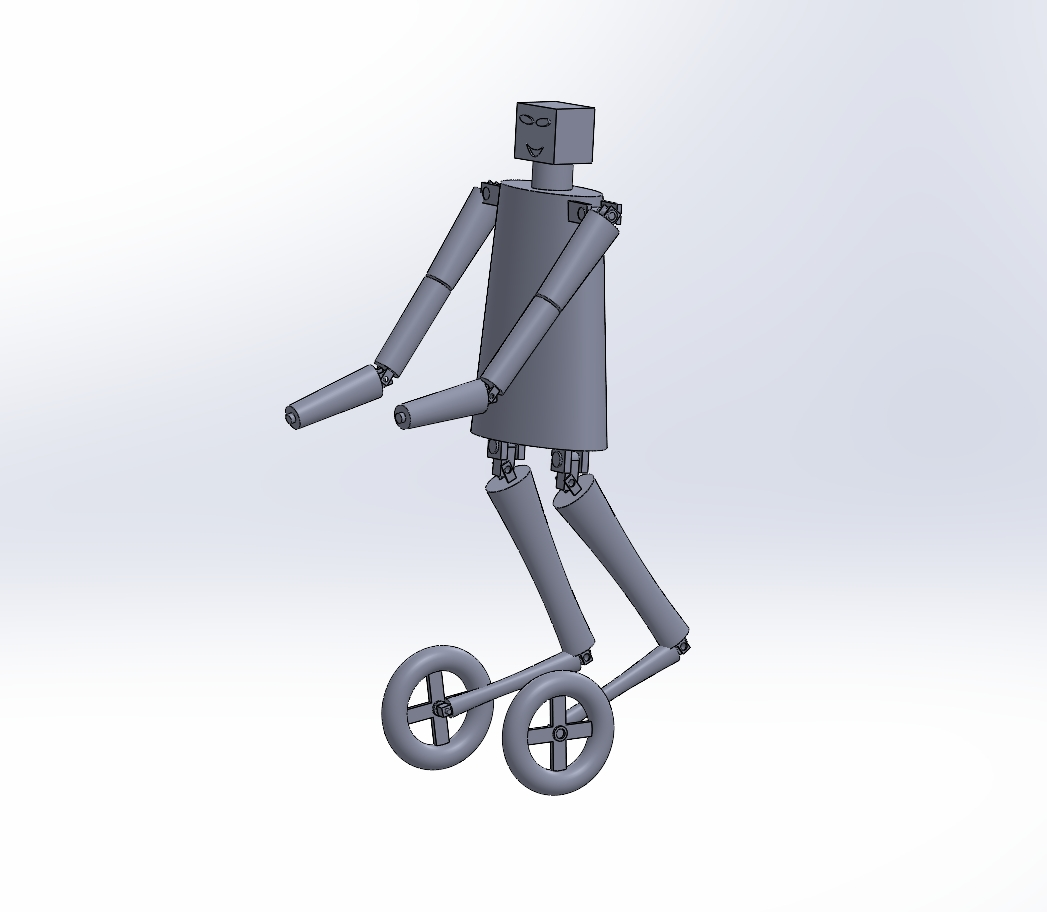
\includegraphics[width=0.45\linewidth]{wheeled_humanoid.png}}
  \caption{三种构想机器人类型的示意图汇总}
  \label{fig:multi_image}
\end{figure}

如图\ref{fig:multi_image}所示,这里给出几种近来构想的机器人结构草图和简单介绍,可以作为随后研究的机器人备选平台参考。

\section[弹跳轮足+机械手机器人]{弹跳轮足+机械手机器人}
如图\ref{fig:wheeled_humanoid}所示,该类型的机器人由类似于Ascento\cite[p1]{Klemm_Morra_Salzmann_Tschopp_Bodie_Gulich_Kung_Mannhart_Pfister_Vierneisel_et_al_2019}类型机器人的双轮足,在此基础上添加两个机械臂构成类人形机器人。该类型的机器人可以轮式地行走和跳跃,同时可以用机械臂模仿双手进行各种操作。

% \textcolor{red}{\small
% 待补充示意图片...
% }
\begin{figure}
  \centering
  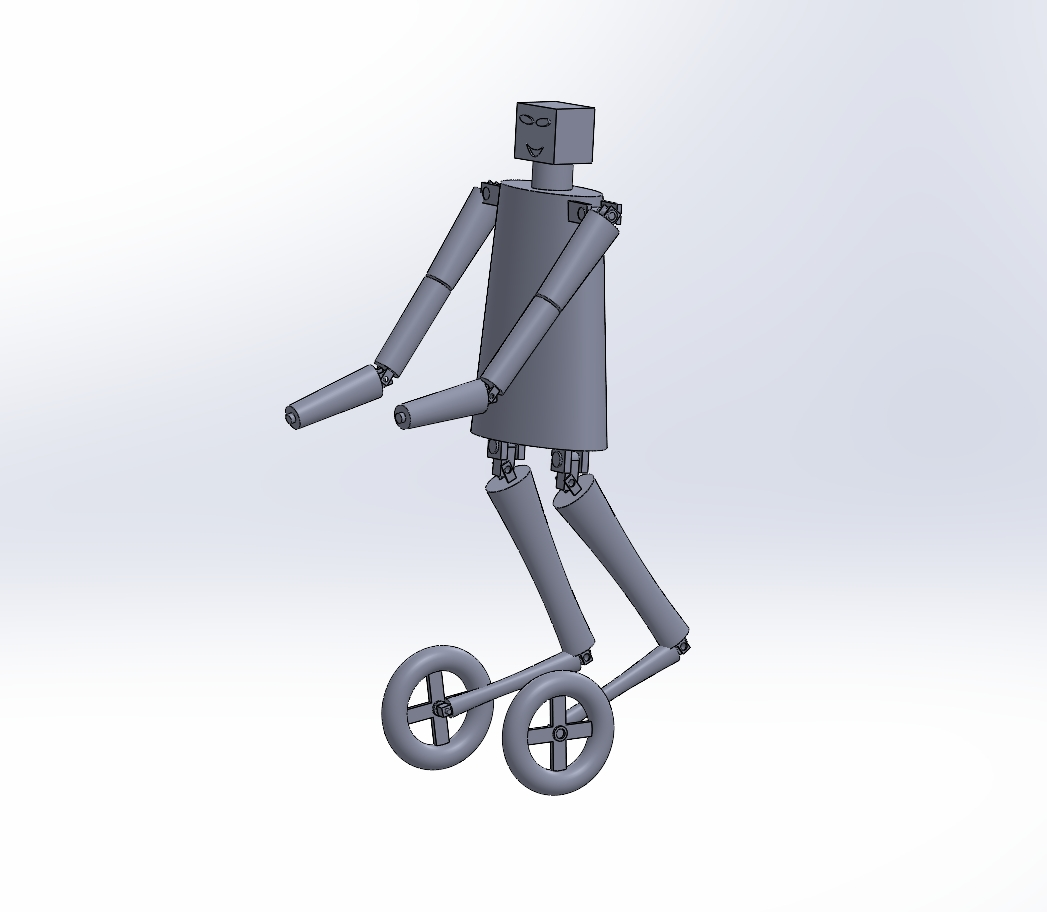
\includegraphics[width=0.6\linewidth]{wheeled_humanoid.png}
  \caption[wheeled_humanoid]{Schematic view of wheeled-humanoid robot}
  \label{fig:wheeled_humanoid}
\end{figure}

该类型机器人的控制基础是倒立摆模型和机械臂运动学,它相对于现有双轮机器人,如Ascento\cite[p1]{Klemm_Morra_Salzmann_Tschopp_Bodie_Gulich_Kung_Mannhart_Pfister_Vierneisel_et_al_2019}等,新的控制问题难点是:
\begin{enumerate}
  \item 在机械手运动的同时保持双轮足的稳定,比如从空手到搬起重物的过程;
  \item 如何让手臂配合轮足实现更加灵巧和优雅的动作;
\end{enumerate}

\section[轮鞋足式+机械手机器人]{轮鞋足式+机械手机器人}
如图\ref{fig:roller_humanoid}所示,该类型的机器人由类似一般人形机器人的基本结构,在此基础之上为每个脚添加四个轮子

% \textcolor{red}{\small
% 待补充示意图片...
% }
\begin{figure}
  \centering
  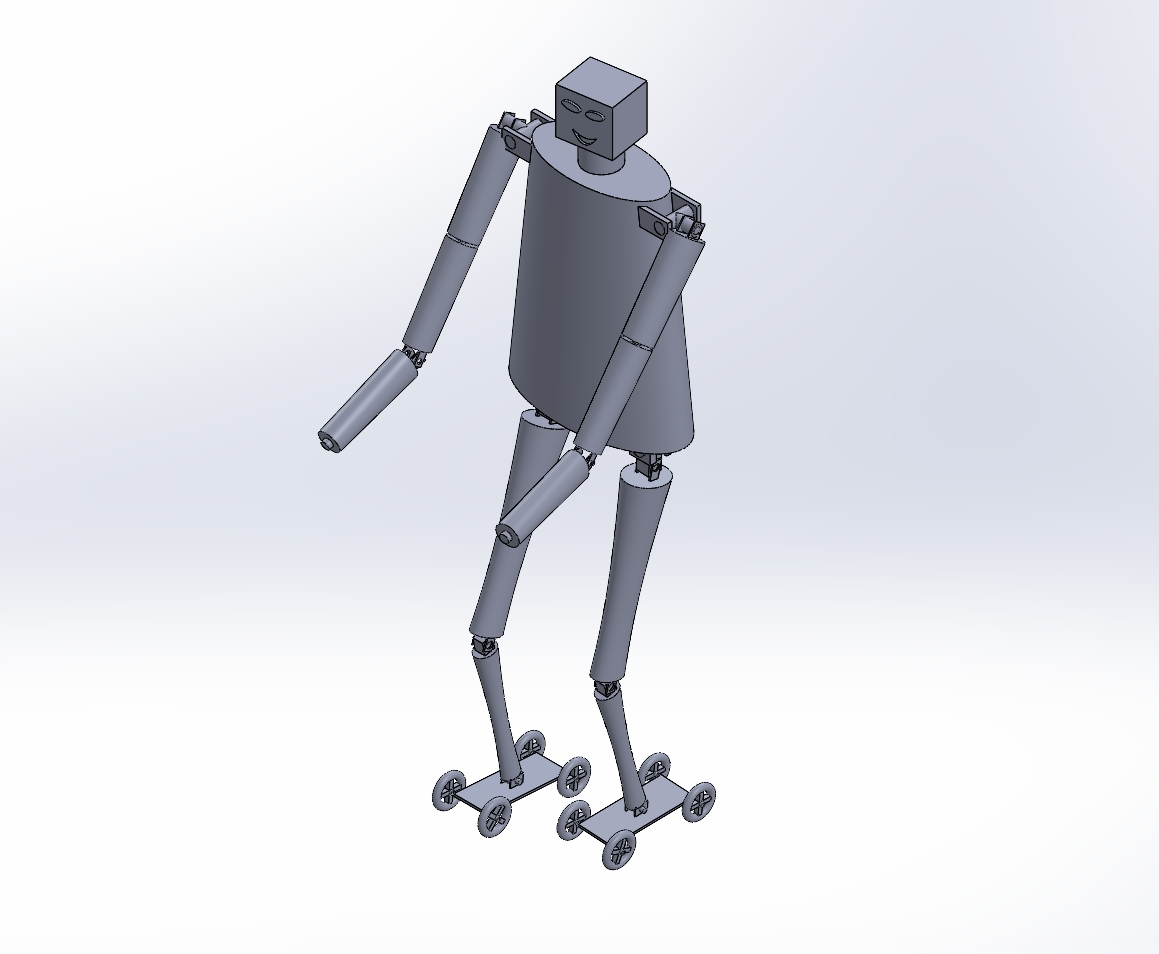
\includegraphics[width=0.6\linewidth]{roller_humanoid.png}
  \caption[roller_humanoid]{Schematic view of roller humanoid.}
  \label{fig:roller_humanoid}
\end{figure}

该类型机器人的控制基础是ZMP约束和机械臂运动学,它相对于现有人形机器人,如\cite[p]{Herzog_Rotella_Schaal_Righetti_2015, Dietrich_Bussmann_Petit_Kotyczka_Ott_Lohmann_Albu_Schäffer_2015}等,新的控制问题难点是:
\begin{enumerate}
  \item 如何实现步态和轮式之间的运动切换;
  \item 如何实现步态和轮式的联合运动平衡;
  \item 在上面两点的基础上,如何结合机械臂实现更加灵巧、优雅、节能的动作;
\end{enumerate}

\section[弹跳轮足+飞行器机器人]{弹跳轮足+飞行器机器人}
如图\ref{fig:wheeled_flying}所示,该类型的机器人由类似于Ascento\cite[p1]{Klemm_Morra_Salzmann_Tschopp_Bodie_Gulich_Kung_Mannhart_Pfister_Vierneisel_et_al_2019}类型机器人的双轮足,在此基础之上添加一对旋翼使其具备飞行能力。

% \textcolor{red}{\small
% 待补充示意图片...
% }
\begin{figure}
  \centering
  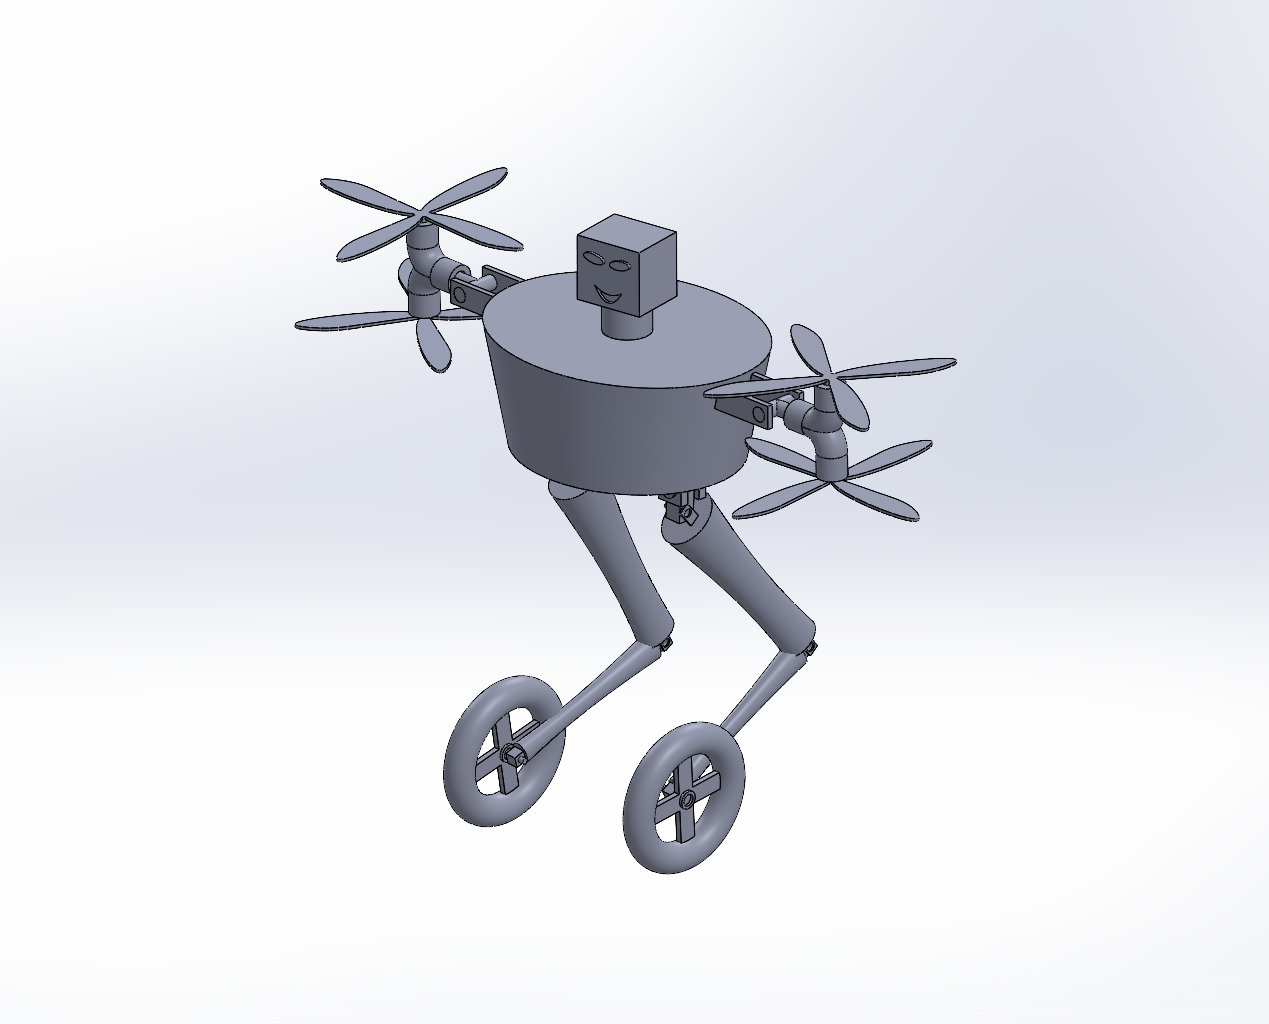
\includegraphics[width=0.6\linewidth]{wheeled_flying.png}
  \caption[short]{Schematic view of wheeled-flying robot.}
  \label{fig:wheeled_flying}
\end{figure}

该类型机器人的控制基础是倒立摆模型和飞行器控制,它相对于现有双轮机器人,如Ascento\cite[p1]{Klemm_Morra_Salzmann_Tschopp_Bodie_Gulich_Kung_Mannhart_Pfister_Vierneisel_et_al_2019}等,新的控制问题难点是:
\begin{enumerate}
  \item 飞行器的矢量控制;
  \item 如何优化设计使得旋翼提供的升力可以满足飞行控制
  \item 续航安全问题;
  \item 如何让旋翼配合轮足实现更加灵巧、优雅、节能、稳定的动作;
\end{enumerate}

% \section[机械狗+飞行器机器人]{机械狗+飞行器机器人}
% 该类型的机器人由类似于ANYmal\cite[p1]{Hwangbo_Lee_Dosovitskiy_Bellicoso_Tsounis_Koltun_Hutter_2019}类型机器人的四足机器人,在此基础之上添加两对旋翼使其具备飞行能力。

% \textcolor{red}{\small
% 待补充示意图片...
% }

% 该类型机器人的控制基础是ZMP约束和飞行器控制,它相对于现有双轮机器人,如Ascento\cite[p1]{Klemm_Morra_Salzmann_Tschopp_Bodie_Gulich_Kung_Mannhart_Pfister_Vierneisel_et_al_2019}等,新的控制问题难点是:
% \begin{enumerate}
%   \item 飞行器的矢量控制;
%   \item 如何优化设计使得旋翼提供的升力可以满足飞行控制
%   \item 续航安全问题;
%   \item 如何让旋翼配合轮足实现更加灵巧、优雅、节能、稳定的动作;
% \end{enumerate}

